%
% Template Laporan Tugas Akhir Jurusan Informatika Unsyiah 
%
% @author Abdul Hafidh
% @version 1.1
% @since 08.09.2023
%
% Template ini telah disesuaikan dengan aturan penulisan tugas akhir 
% yang terdapat pada dokumen Panduan Tugas Akhir FMIPA Unsyiah tahun 2016.
%

% karena jifhasiltheme.cls ada di folder lib, maka kita harus menambahkan path lib/ ke dalam path pencarian file
\makeatletter
\def\input@path{{lib/}}
\makeatother
% Template pembuatan naskah tugas akhir.
\documentclass[dvipsnames]{jifhasiltheme-final}

\tolerance=1
\emergencystretch=\maxdimen
\hyphenpenalty=10000
\hbadness=10000

% Karena file hype.indonesia.tex ada di folder language, tambah path pencarian file
\makeatletter
\def\input@path{{language/}}
\makeatother
%
% Hyphenation untuk Indonesia 
%
% @author  Andreas Febrian
% @version 1.00
% 
% Tambahkan cara pemenggalan kata-kata yang salah dipenggal secara otomatis 
% oleh LaTeX. Jika kata tersebut dapat dipenggal dengan benar, maka tidak 
% perlu ditambahkan dalam berkas ini. Tanda pemenggalan kata menggunakan 
% tanda '-'; contoh:
% menarik
%   --> pemenggalan: me-na-rik
%

\hyphenation{
    % alphabhet A
    a-na-li-sa a-tur 
    a-pli-ka-si 
    android
    % alphabhet B
    ba-ngun-an 
    be-be-ra-pa 
    ber-ge-rak
    ber-ke-lan-jut-an 
    ber-pe-nga-ruh 
    % alphabhet C
    ca-ri
    % alphabhet D
    di-sim-pan di-pim-pin de-ngan da-e-rah di-ba-ngun da-pat di-nya-ta-kan 
    di-sim-bol-kan di-pi-lih di-li-hat de-fi-ni-si
    % alphabhet E
    e-ner-gi eks-klu-sif
    % alphabhet F
    fa-si-li-tas
    foot-print
    % alphabhet G
    ga-bung-an ge-rak
    % alphabhet H
    ha-lang-an
    % alphabhet I
    % alphabhet J
    % alphabhet K
    ke-hi-lang-an
    ku-ning 
    kua-li-tas ka-me-ra ke-mung-kin-an ke-se-pa-ham-an
    % alphabhet L
    ling-kung-an
    % alphabhet M
    me-neng-ah
    meng-a-tas-i me-mung-kin-kan me-nge-na-i me-ngi-rim-kan 
    meng-u-bah meng-a-dap-ta-si me-nya-ta-kan mo-di-fi-ka-si
    meng-a-tur
    mem-pro-mo-si-kan
    me-la-ku-kan
    meng-i-den-ti-fi-ka-si-kan
    % alphabhet N
    nya-ta non-eks-klu-sif
    % alphabhet O
    % alphabhet P
	pe-nye-rap-an 
	pe-ngon-trol
    pe-mo-del-an
    pe-ran  pe-ran-an-nya
    pem-ba-ngun-an pre-si-den pe-me-rin-tah prio-ri-tas peng-am-bil-an 
    peng-ga-bung-an pe-nga-was-an pe-ngem-bang-an 
    pe-nga-ruh pa-ra-lel-is-me per-hi-tung-an per-ma-sa-lah-an 
    pen-ca-ri-an peng-struk-tur-an
    pe-ran-ca-ngan
    plat-form
    patch
    % alphabhet Q
    % alphabhet R
    ran-cang-an
    % alphabhet S
    si-mu-la-si sa-ngat
    smart-phone
    % alphabhet T
    te-ngah
    ter-da-pat
    % alphabhet U
    % alphabhet V
    % alphabhet W
    % alphabhet X
    % alphabhet Y
    % alphabhet Z
    % special
}

% Untuk prefiks pada daftar gambar dan tabel
\usepackage[titles]{tocloft}

\usepackage{etoolbox}% http://ctan.org/pkg/etoolbox
\makeatletter
\patchcmd{\@chapter}{\addtocontents{lof}{\protect\addvspace{10\p@}}}{}{}{} % LoF
\patchcmd{\@chapter}{\addtocontents{lot}{\protect\addvspace{10\p@}}}{}{}{} % LoT
\makeatother

\usepackage[justification=centering]{caption} % atau misalnya [format=hang]
\usepackage{amssymb}
% Tambahan dari Budi
\newcommand*{\enableboldchapterintoc}{%
  \addtocontents{toc}{\string\renewcommand{\protect\cftchapfont}{\protect\normalfont\protect\bfseries}}%
  \addtocontents{toc}{\string\renewcommand{\protect\cftchappagefont}{\protect\normalfont\protect}}%
  \addtocontents{toc}{\protect\setlength{\cftbeforechapskip}{12pt}}%
}
\newcommand*{\disableboldchapterintoc}{%
  \addtocontents{toc}{\string\renewcommand{\protect\cftchappagefont}{\protect\normalfont}}%
  \addtocontents{toc}{\string\renewcommand{\protect\cftchapfont}{\protect\normalfont}}%
  \addtocontents{toc}{\protect\setlength{\cftbeforechapskip}{0pt}}%
}
% End tambahan dari Budi

\renewcommand{\cftdotsep}{0.5}
\renewcommand{\cftchapleader}{\cftdotfill{\cftdotsep}}

\renewcommand\cftfigpresnum{Gambar\  }
\renewcommand\cfttabpresnum{Tabel\   }

\newcommand{\listappendicesname}{DAFTAR LAMPIRAN}
\newlistof{appendices}{apc}{\listappendicesname}
\newcommand{\appendices}[1]{\addcontentsline{apc}{appendices}{#1}}
\newcommand{\newappendix}[1]{\section*{#1}\appendices{#1}}

% Untuk hyperlink dan table of content
\usepackage[hidelinks]{hyperref}
\renewcommand\UrlFont{\rmfamily\itshape}
\newlength{\mylenf}
\settowidth{\mylenf}{\cftfigpresnum}
\setlength{\cftfignumwidth}{\dimexpr\mylenf+2em}
\setlength{\cfttabnumwidth}{\dimexpr\mylenf+2em}

% Agar ada tulisan BAB pada TOC
\renewcommand\cftchappresnum{BAB } 
\cftsetindents{chapter}{0em}{4.5em}
\cftsetindents{section}{4.5em}{2em}
\cftsetindents{subsection}{6.5em}{3em}

\renewcommand{\cftsecaftersnum}{.}
\renewcommand{\cftsubsecaftersnum}{.}

\addtocontents{toc}{~\hfill \textit{Halaman}\par}
\addtocontents{lof}{~\hfill \textit{Halaman}\par}
\addtocontents{lot}{~\hfill \textit{Halaman}\par}
\addtocontents{apc}{~\hfill \textit{Halaman}\par}

% Untuk judul section
\usepackage{titlesec}
\titlelabel{\thetitle.\quad}

% Untuk caption dengan titik sebagai pemisah
\usepackage[labelsep=period]{caption}
\usepackage[labelfont=bf]{caption}
\usepackage{subcaption}

\usepackage{color} % untuk warna
\usepackage{longtable}
\usepackage{pdflscape}
\usepackage{lscape}
% Agar bisa menulis code snippet
\usepackage{lstautogobble} % it's me!
\usepackage{listings}
\usepackage{xcolor}  % Untuk warna sintaks (opsional)
\usepackage{inconsolata}  % Font monospace yang rapi (disarankan)
\usepackage{adjustbox}
% Konfigurasi dasar untuk listings
\lstset{
    basicstyle=\ttfamily\small,       % Gunakan font monospace (Inconsolata)
    keywordstyle=\color{blue},        % Warna keyword (biru)
    commentstyle=\color{gray},        % Warna komentar (abu-abu)
    stringstyle=\color{red},          % Warna string (merah)
    numbers=left,                     % Tampilkan nomor baris di kiri
    numberstyle=\tiny\color{gray},    % Gaya nomor baris
    stepnumber=1,                     % Interval nomor baris
    tabsize=4,                        % Ukuran tab
    showstringspaces=false,           % Jangan tunjukkan spasi di string
    breaklines=true,                  % Potong baris panjang
    frame=single,                     % Bingkai sekitar kode
    rulecolor=\color{lightgray},      % Warna bingkai
    backgroundcolor=\color{white},    % Warna latar belakang
    literate=                         % Handle karakter khusus
        {á}{{\'a}}1 {é}{{\'e}}1 {í}{{\'i}}1 {ó}{{\'o}}1 {ú}{{\'u}}1
        {Á}{{\'A}}1 {É}{{\'E}}1 {Í}{{\'I}}1 {Ó}{{\'O}}1 {Ú}{{\'U}}1
        {à}{{\`a}}1 {è}{{\`e}}1 {ì}{{\`i}}1 {ò}{{\`o}}1 {ù}{{\`u}}1
        {À}{{\`A}}1 {È}{{\'E}}1 {Ì}{{\`I}}1 {Ò}{{\`O}}1 {Ù}{{\`U}}1
        {ä}{{\"a}}1 {ë}{{\"e}}1 {ï}{{\"i}}1 {ö}{{\"o}}1 {ü}{{\"u}}1
        {Ä}{{\"A}}1 {Ë}{{\"E}}1 {Ï}{{\"I}}1 {Ö}{{\"O}}1 {Ü}{{\"U}}1
        {â}{{\^a}}1 {ê}{{\^e}}1 {î}{{\^i}}1 {ô}{{\^o}}1 {û}{{\^u}}1
        {Â}{{\^A}}1 {Ê}{{\^E}}1 {Î}{{\^I}}1 {Ô}{{\^O}}1 {Û}{{\^U}}1
        {œ}{{\oe}}1 {Œ}{{\OE}}1 {æ}{{\ae}}1 {Æ}{{\AE}}1 {ß}{{\ss}}1
        {ç}{{\c c}}1 {Ç}{{\c C}}1 {ø}{{\o}}1 {å}{{\r a}}1 {Å}{{\r A}}1
        {€}{{\euro}}1 {£}{{\pounds}}1
}
\lstset{autogobble=true}
% Contoh bahasa yang didukung (sesuaikan dengan kebutuhan)
\lstdefinestyle{Java}{
    language=Java,
    morekeywords={String, interface, implements, class}
}

\lstdefinestyle{Python}{
    language=Python,
    keywordstyle=\color{teal}
}
\usepackage{caption} % Untuk kustomisasi caption
%Gaya Caption
\captionsetup[lstlisting]{
    labelfont=md,          % Label tidak bold
    textfont=md,           % Teks caption tidak bold
    singlelinecheck=true,  % Centang caption 1 baris
    justification=raggedright, % Rata kiri untuk multi-baris
    labelsep=space,
    format=hang,              % Format "hang" untuk indentasi
    indention=0pt             % Hapus indentasi pada baris kedua+
}
%untuk definisi teorema
\usepackage{amsthm}

% Definisi lingkungan teorema
\theoremstyle{plain}
\newtheorem{theorem}{Teorema}[section]
\newtheorem{corollary}[theorem]{Korolari}

\theoremstyle{definition}
\newtheorem{definition}{Definisi}[section]

\theoremstyle{remark}
\newtheorem*{remark}{Catatan}
% Contoh definisi untuk lingkungan "example"
\theoremstyle{definition} % Gaya: teks normal, judul tebal
\newtheorem{example}{Contoh}[section] % Nomor mengikuti bagian
\usepackage{adjustbox}
\usepackage{fancybox, graphicx} % shadow gambar
\usepackage{url}
\usepackage{microtype}
\usepackage{siunitx}
\usepackage{xcolor}
\usepackage{multirow}
\usepackage[normalem]{ulem}
\useunder{\uline}{\ul}{}
\usepackage{array}
\newcolumntype{P}[1]{>{\centering\arraybackslash}p{#1}}
\newcolumntype{M}[1]{>{\centering\arraybackslash}m{#1}}

\makeatletter
\def\input@path{{include/}}
\makeatother

% Sampul Depan
%-----------------------------------------------------------------
% Sampul Depan
%-----------------------------------------------------------------
\judulcover{Analisis Prediktif Spektrum Emisi \textit{Laser-Induced Breakdown Spectroscopy} (LIBS) Multi-Elemen Berbasis Simulasi Sintetis dengan Informer}

\judul{Analisis Prediktif Spektrum Emisi \textit{Laser-Induced Breakdown Spectroscopy} (LIBS) Multi-Elemen Berbasis Simulasi Sintetis dengan Informer}
\judulinggris{Predictive Analysis of Multi-Element Laser-Induced Breakdown Spectroscopy (LIBS) Emission Spectra Based on Synthetic Simulation with Informer}

% nama lengkap
\fullname{Birrul Walidain }

% NPM (Nomor Pokok Mahasiswa)
\idnum{2008102010010}

\degree{Sarjana Sains}

\yearsubmit{Mei, 2025}

\dept{Fisika}

\prodi{Sarjana Fisika}

% Pembimbing Pertama
\firstsupervisor{Prof. Dr. Eng. Nasrullah, S.Si., M.T.}
\firstnip{197607031995121001}
\firstdept{Fisika}

% Pembimbing Kedua
\secondsupervisor{Dr. Khairun Saddami, S.T.}
\secondnip{199103182022031008}
\seconddept{Teknik Komputer}
% Ketua Jurusan
\kajur{Dr. Saumi Syahreza, S.Si., M.Si.}
\kajurnip{197609172005011002}

% Dekan Fakultas
\dekan{Prof. Dr. Taufik Fuadi Abidin, S.Si., M.Tech.}
\dekannip{197010081994031002}

%kaprodi
\kaprodi{Dr. Saumi Syahreza, S.Si., M.Si.}
\kaprodinip{197609172005011002}

\koorta{Zulfalina, S.Si., M.Si.}
\koortanip{197507072002122001}
% tangal lulus proposal, seminar hasil atau sidang
\approvaldate{Kamis, 14 Mei 2024}

%-----------------------------------------------------------------
% End of Sampul Depan
%-----------------------------------------------------------------


% Awal dokumen
\usepackage{fancyhdr}
\usepackage{rotating}
% Untuk daftar program
\makeatletter
\begingroup\let\newcounter\@gobble\let\setcounter\@gobbletwo
\globaldefs\@ne \let\c@loldepth\@ne
\newlistof{listings}{lol}{\lstlistlistingname}
\endgroup
\let\l@lstlisting\l@listings
\AtBeginDocument{\addtocontents{lol}{\protect\addvspace{10\p@}}}
\makeatother
\renewcommand{\lstlistoflistings}{\listoflistings}
\renewcommand\cftlistingspresnum{Program~}
\cftsetindents{listings}{1.5em}{7em}

% Tab untuk daftar pustaka
\setlength{\bibhang}{30pt}
\usepackage{pdfpages}
\usepackage[table,xcdraw]{xcolor} % Jika diperlukan, pastikan xcdraw hanya dimuat sekali
\usepackage{colortbl}

\begin{document}
\sloppy
\fancyhf{} 
\fancyfoot[C]{\thepage}

\cover
\approvalpage

\bplagiasi % Note: \preface JANGAN DIHAPUS!
\onehalfspacing
\noindent
Saya yang bertanda tangan di bawah ini,

\vspace{0.2cm}
\noindent
\begin{center}
	\begin{tabularx}{0.9\textwidth}{@{} l X @{}} % Gunakan X untuk kolom yang menyesuaikan lebar
		Nama lengkap          & : Birrul Walidain \\
		Tempat/tanggal lahir  & : Lhokseumawe/11 November 2002 \\
		NPM                   & : 2008102010010 \\
		Program Studi         & : Fisika \\
		Fakultas              & : MIPA \\
		Judul Tugas Akhir     & : 
		\begin{tabular}[t]{@{}p{\linewidth}@{}}
			IDENTIFIKASI MULTI ELEMEN PADA SPEKTRUM EMISI LIBS KOMPLEKS DARI 
			TANAH VULKANIK SEULAWAH AGAM MENGGUNAKAN ALGORITMA 
			\textit{LONG SHORT-TERM MEMORY} (LSTM)
		\end{tabular} \\
	\end{tabularx}
\end{center}



\vspace{0.2cm}
\noindent
Menyatakan dengan sesungguhnya bahwa Laporan Tugas Akhir saya dengan judul di atas adalah \textbf{hasil karya saya sendiri} bersama dosen pembimbing dan \textbf{bebas plagiasi}.

\vspace{0.2cm}
\noindent
Jika ternyata di kemudian hari terbukti bahwa Laporan Tugas Akhir merupakan hasil plagiasi, saya bersedia menerima sanksi yang berlaku di Universitas Syiah Kuala.

\vspace{1cm}
\begin{onehalfspace}
	\begin{flushright} % Rata kanan
		\begin{tabular}{l@{}}
			Banda Aceh, 17 Maret 2025 \\[-0.15cm]
			Yang menyatakan, \\
			\\[1.5cm] % Jarak untuk tanda tangan
			Birrul Walidain \\[-0.15cm]
			NPM. 2008102010010 \\
		\end{tabular}
	\end{flushright}
\end{onehalfspace}


\spernyataan % Note: \preface JANGAN DIHAPUS!

\noindent
Yang bertanda tangan di bawah ini,
\vspace{-0.1cm}
\begin{table}[H]
{\renewcommand{\arraystretch}{0.7}
\begin{tabular}{M{0.6cm}lll}
	&1. 	& Nama   		&: Birrul Walidain \\
	&	& NPM       			&: 2008102010010   \\
	&	& Program Studi  		&: S1-Fisika \\
	&	& Status 				&: Mahasiswa \\  
	&2. 	& Nama  		&: Prof. Dr. Eng. Nasrullah, S.Si., M.T. \\
	&	& NIP       			&: 197607031995121001   \\
	&	& Jurusan/Prodi   		&: Fisika \\
	&	& Status 				&: Pembimbing I \\  
	&3. 	& Nama  		&: Dr. Khairun Saddami, S.T. \\
	&	& NIP       			&: 199103182022031008   \\
	&	& Departemen/Prodi   		&: Teknik Komputer \\
	&	& Status 				&: Pembimbing II   
\end{tabular}
}
\end{table}
\onehalfspacing
\vspace{-0.4cm}
\noindent
Dengan ini menyatakan hasil penelitian Tugas Akhir yang berjudul \textbf{“IDENTIFIKASI MULTI ELEMEN PADA SPEKTRUM EMISI LIBS KOMPLEKS DARI 
TANAH VULKANIK SEULAWAH AGAM MENGGUNAKAN ALGORITMA 
\textit{LONG SHORT-TERM MEMORY} (LSTM)”} tidak dipublikasikan secara \textit{full-text} di sistem ETD (\textit{Electronic Theses and Dissertations}) Universitas Syiah Kuala hingga batas waktu 5 tahun dari tanggal kelulusan.

\vspace{0.4cm}
\noindent
Demikian surat pernyataan ini dibuat dengan sebenarnya untuk dapat dipergunakan seperlunya.

\vspace{0.4cm}
{\renewcommand{\arraystretch}{0.8}
\centering
\begin{tabular}{lll}
	&Darussalam, 14 Mei 2025		& \\
	&Yang membuat pernyataan,			& \\
	&&\\
	Pembimbing I,							&Pembimbing II,							&Mahasiswa,\\
	[1.5cm]
	\underline{Prof. Dr. Eng. Nasrullah, M.T.}	&\underline{Dr. Khairun Saddami, S.T.} &\underline{Birrul Walidain}\\
	NIP. 197607031995121001				&NIP. 199103182022031008				&NPM. 2008102010010\\
	&&\\

\end{tabular}
}

{\renewcommand{\arraystretch}{0.8}
\begin{center}\
	Mengetahui: \\
	\hspace{0.3cm}
	\begin{tabular}{lll}
		Koordinator Program Studi Fisika&\hspace{2.7cm}	&Koordinator TA,\\
		Universitas Syiah Kuala, &&\\
		[1.5cm]
		\underline{Dr. Saumi Syahreza, S.Si., M.Si.}	&&\underline{Zulfalina, S.Si., M.Si.}\\
		NIP. 198008312009122003						&&NIP. 197507072002122001 				
	\end{tabular}
\end{center}

}



\begin{abstractind}

Artificial Neural Networks (ANN) bring important insights to the development of Laser-induced Breakdown Spectroscopy methods in qualitatively identifying spectra, especially soil spectra. Volcanic soils were highly fertile which played a major role in the development of the agrarian industry in Indonesia. Thus, the need for rapid identification techniques to analyze major elements in volcanic soil is the answer to the massive volcanic soil in Indonesia. Long Short-Term Memory (LSTM) was an enhanced variant of conventional Recurrent Neural Network (RNN). In this research, the LSTM model was trained with simulated pure element spectra. These simulated pure elemental spectra were built from various elements with plasma state variance. The model was also built to consider the matrix effect present in experiment. The model was then fine-tuned with spectra of Mount Seulawah Agam volcanic soil taken from three sub-districts: Seulimum, Cot Glie, and Lembah Seulawah with each at a depth of 20cm, 40cm, and 60cm from the ground surface. The LSTM model then successfully predicted several major elements such as Calcium, Aluminium, Iron, Magnesium, and Silica accurately and compared with the X-ray fluorescence (XRF) analysis method technique. This research makes an important contribution to the use of ANN for geochemical analysis of volcanic activity in Indonesia for further utilization.

\bigskip
\noindent
\textbf{Kata kunci :} lorem ipsum dolor sit amet
\end{abstractind} 
\begin{abstracteng}
\textit{Artificial Neural Networks (ANN) bring important insights to the development of Laser-induced Breakdown Spectroscopy methods in qualitatively identifying spectra, especially soil spectra. Volcanic soils were highly fertile which played a major role in the development of the agrarian industry in Indonesia. Thus, the need for rapid identification techniques to analyze major elements in volcanic soil is the answer to the massive volcanic soil in Indonesia. Long Short-Term Memory (LSTM) was an enhanced variant of conventional Recurrent Neural Network (RNN). In this research, the LSTM model was trained with simulated pure element spectra. These simulated pure elemental spectra were built from various elements with plasma state variance. The model was also built to consider the matrix effect present in experiment. The model was then fine-tuned with spectra of Mount Seulawah Agam volcanic soil taken from three sub-districts: Seulimum, Cot Glie, and Lembah Seulawah with each at a depth of 20cm, 40cm, and 60cm from the ground surface. The LSTM model then successfully predicted several major elements such as Calcium, Aluminium, Iron, Magnesium, and Silica accurately and compared with the X-ray fluorescence (XRF) analysis method technique. This research makes an important contribution to the use of ANN for geochemical analysis of volcanic activity in Indonesia for further utilization.
}

\bigskip
\noindent
\textbf{Kata kunci :} lorem, ipsum, dolor, sit, amet
\end{abstracteng} 

% Kata pengantar
\preface % Note: \preface JANGAN DIHAPUS!


Segala puji dan syukur kehadiran Allah SWT yang telah melimpahkan rahmat dan hidayah-Nya kepada kita semua, sehingga penulis dapat menyelesaikan penulisan Tugas Akhir yang berjudul \textbf{{\MakeUppercase{Identifikasi Multi Elemen pada Spektrum Emisi LIBS Kompleks Dari Tanah Vulkanik Seulawah Agam Menggunakan Algoritma \textit{Long Short-Term Memory} (LSTM)}}} yang telah dapat diselesaikan sesuai rencana. Penulis banyak mendapatkan berbagai pengarahan, bimbingan, dan bantuan dari berbagai pihak. Oleh karena itu, melalui tulisan ini penulis mengucapkan rasa terima kasih kepada:

\begin{enumerate} 

	\item {Bapak Dr. Saumi Syahreza, S.Si., M.Si. selaku Ketua Departemen Fisika Fakultas MIPA Universitas Syiah Kuala.}

	\item{Bapak Prof. Dr. Eng. Nasrullah, S.Si., M.T.
 selaku Dosen Pembimbing I yang telah banyak memberikan bimbingan dan arahan kepada penulis, sehingga penulis dapat menyelesaikan Tugas Akhir ini.}
	\item{Bapak Dr. Khairun Saddami, S.T.
 selaku Dosen Pembimbing II yang telah banyak memberikan bimbingan dan arahan kepada penulis, sehingga penulis dapat menyelesaikan Tugas Akhir ini.}

	\item{Bapak Dr. Kurnia Lahna, M.T. selaku Dosen Wali yang telah membimbing
dan memberikan motivasi kepada penulis selama masa perkuliahan.}
  	%\item{Ayah dan Ibu sebagai kedua orang tua penulis yang senantiasa selalu mendukung aktivitas dan kegiatan yang penulis lakukan baik secara moral maupun material serta menjadi motivasi terbesar bagi penulis untuk menyelesaikan Tugas Akhir ini.}
	%\item{Seluruh Dosen di Departemen Fisika Fakultas MIPA atas ilmu dan didikannya selama perkuliahan.}
	%\item{Sahabat dan teman-teman seperjuangan Departemen Fisika USK 2020 lainnya.}
\end{enumerate}

%\vspace{1.5cm}

Penulis juga menyadari segala ketidaksempurnaan yang terdapat didalamnya baik dari segi materi, cara, ataupun bahasa yang disajikan. Seiring dengan ini penulis mengharapkan kritik dan saran dari pembaca yang sifatnya dapat berguna untuk kesempurnaan Tugas Akhir ini. Harapan penulis semoga tulisan ini dapat bermanfaat bagi banyak pihak dan untuk perkembangan ilmu pengetahuan.

\vspace{1cm}


\begin{tabular}{p{7.5cm}l}
	&Banda Aceh, 14 Agustus 2024\\
	&\\
	&\\
	&\multirow{1.5}{7.5cm}{\underline{Birrul Walidain}} \\ 
	&NPM. 2008102010010 \\
\end{tabular}


\titleformat{\section}{\normalfont\bfseries\uppercase}{\thesection}{1.7em}{}
\titleformat{\subsection}{\normalfont\bfseries}{\thesubsection}{0.9em}{}

\addcontentsline{toc}{chapter}{Daftar Isi}
\begin{singlespace}
  \tableofcontents
\end{singlespace}
\listoftables
\addcontentsline{toc}{chapter}{Daftar Tabel}
\listoffigures
\addcontentsline{toc}{chapter}{Daftar Gambar}
\listofappendices
\addcontentsline{toc}{chapter}{Daftar Lampiran}

\enableboldchapterintoc

% File: include/simbol.tex
% Daftar simbol fisika dan matematika yang digunakan dalam dokumen.
% Diurutkan berdasarkan abjad.

\chapter*{DAFTAR SIMBOL}
\addcontentsline{toc}{chapter}{Daftar Simbol}

\begin{itemize}
    \item[$A_{ki}$] : Probabilitas transisi spontan (Koefisien Einstein A).
    \item[$\mathcal{A}$] : Kamus (dictionary) himpunan bagian atom.
    \item[$\alpha_G$] : Lebar profil garis Gaussian (Doppler).
    \item[$\alpha_L$] : Lebar profil garis Lorentzian (Stark/Pressure).
    \item[$\approx$] : Simbol kira-kira sama dengan.
    \item[$c$] : Kecepatan cahaya dalam vakum.
    \item[$\mathcal{C}$] : Himpunan atom kandidat.
    \item[$\mathcal{D}$] : Dataset transisi atom.
    \item[$\Delta$] : Simbol selisih atau perbedaan (Delta).
    \item[$\partial$] : Operator turunan parsial.
    \item[$E$] : Energi, khususnya tingkat energi atom ($E_i, E_k$).
    \item[$\exp()$] : Fungsi eksponensial.
    \item[$f$] : Fraksi populasi ($f_{\text{ion}}, f_{\text{neutral}}$).
    \item[$g$] : Berat statistik atau degenerasi tingkat energi.
    \item[$h$] : Konstanta Planck.
    \item[$I$] : Intensitas garis spektral.
    \item[$\mathcal{I}$] : Kamus intensitas sementara.
    \item[$\int$] : Operator integral.
    \item[$k_B$] : Konstanta Boltzmann.
    \item[$\lambda$] : Panjang gelombang transisi spektral ($\lambda_{ij}$).
    \item[$\log()$] : Fungsi logaritma.
    \item[$m_e$] : Massa elektron.
    \item[$n_e$] : Kerapatan elektron (electron density).
    \item[$N$] : Jumlah atau kerapatan partikel ($N_{\text{ion}}, N_{\text{neutral}}$).
    \item[$\nabla$] : Operator Nabla (del).
    \item[$\propto$] : Simbol sebanding dengan.
    \item[$\mathcal{R}$] : Kamus rasio populasi.
    \item[$\rho$] : Kerapatan (densitas).
    \item[$\mathcal{S}$] : Himpunan data spektrum final.
    \item[$\sigma$] : Tampang lintang (cross-section) atau deviasi standar.
    \item[$\sqrt{}$] : Akar kuadrat.
    \item[$\sum$] : Operator penjumlahan (Sigma).
    \item[$T$] : Temperatur plasma atau gas.
    \item[$Z$] : Fungsi partisi.
\end{itemize}


\renewcommand{\thelstlisting}{\arabic{chapter}.\arabic{lstlisting}}
\renewcommand*\lstlistingname{Program}

\begin{onehalfspace}
\fancyhf{} 
\fancyfoot[C]{\thepage}
\pagenumbering{arabic}

\captionsetup[figure]{labelfont={normalfont}, textfont={normalfont},     singlelinecheck=false,    % Nonaktifkan penengahan otomatis
justification=raggedright, % Rata kiri penuh
labelsep=space,           % Spasi antara label dan teks
format=hang,              % Format "hang" untuk indentasi
indention=0pt, skip=10pt } % Unbold caption gambar
\captionsetup[table]{labelfont={normalfont}, textfont={normalfont}, 
singlelinecheck=false,    % Nonaktifkan penengahan otomatis
justification=raggedright, % Rata kiri penuh
labelsep=space,           % Spasi antara label dan teks
format=hang,              % Format "hang" untuk indentasi
indention=0pt, skip=10pt } % Unbold caption tabel

\fancyhf{} 
\fancyfoot[R]{\thepage}






\chapter{PENDAHULUAN}



\section{Latar Belakang}


\par  Spektroskopi secara sederhana merupakan  interaksi antara materi dan radiasi elektromagnetik yang dapat memberi informasi bagaimana materi menyerap, memancarkan, atau menghamburkan cahaya. Kemudian interaksi ini  digunakan untuk mengidentifikasi dan mengukur komposisi, struktur, dan sifat materi tersebut \parencite{hollas2013}.  
Sejak penemuan garis spektral oleh Fraunhofer dan Kirchhoff, spektroskopi telah menjadi dasar analisis kimia modern, termasuk dalam \textit{Laser-Induced Breakdown Spectroscopy} (LIBS) \parencite{thorne1999}. LIBS menggunakan laser berenergi tinggi untuk menciptakan plasma pada permukaan sampel, menghasilkan spektrum emisi yang kaya informasi. Teknik ini menawarkan analisis cepat dan serbaguna untuk aplikasi seperti identifikasi material dan analisis lingkungan \parencite{thorne1999}.
\begin{figure}
    \centering
    \includegraphics[width=0.8\textwidth]{images/1-latar.jpg}
    \caption{Spekrum mentah (a) pra-pemrosesan (b) spektrum Hidrogen sebelum diberi \textit{noise} (c) dan sesudah diberi \textit{noise} (d) \citep{Gasior2023}}
    \label{fig:kenapa}
\end{figure}

\par \textit{Laser-Induced Breakdown Spectroscopy} (LIBS) adalah teknik analisis yang melibatkan penggunaan laser berenergi tinggi yang kemudian difokuskan ke permukaan sampel untuk menciptakan plasma. LIBS menunjukkan potensinya sebagai teknik analisis yang cepat dan serbaguna untuk berbagai aplikasi, termasuk analisis material. Namun, kompleksitas spektrum LIBS, yang dipengaruhi oleh efek matriks dan fluktuasi plasma, menyulitkan analisis kualitatif dan kuantitatif seperti gambar \ref{fig:kenapa} \parencite{gasior2023analysis}. Metode tradisional, seperti perhitungan numerik berdasarkan persamaan Saha, memerlukan komputasi intensif dan kurang efektif dalam menangani spektrum multi-elemen dengan noise tinggi. Pendekatan pembelajaran mesin, seperti jaringan saraf tiruan (JST) dan pembelajaran mendalam, menunjukkan potensi untuk mengatasi tantangan ini, tetapi memerlukan dataset besar yang mahal untuk dilatih \parencite{gasior2023analysis}. Simulasi spektrum elemen murni dengan profil \textit{Gaussian}, berdasarkan distribusi Boltzmann dan persamaan Saha, dapat menghasilkan dataset sintetis untuk melatih model secara efisien \parencite{pan-2024}. Distribusi Boltzmann memungkinkan perhitungan distribusi energi atom pada suhu tertentu, sementara persamaan Saha menghubungkan fraksi ionisasi dengan suhu dan densitas elektron, membentuk dasar simulasi spektrum LIBS \parencite{thorne1999}.

\par Algoritma Transformer, yang diperkenalkan oleh \cite{vaswani-2017}, unggul dalam memproses data sekuens secara paralel melalui mekanisme \textit{self-attention}. Transformer juga telah berhasil diterapkan dalam dekonvolusi spektrum inframerah dengan \textit{sparse self-attention} oleh \cite{gao2024}, namun aplikasinya untuk simulasi spektrum LIBS berbasis model fisika masih terbatas. Penelitian ini mengusulkan penggunaan Transformer untuk mempelajari spektrum atom yang disimulasikan, dengan memanfaatkan distribusi Boltzmann dan persamaan Saha, guna meningkatkan akurasi prediksi spektrum multi-elemen.


\section{Rumusan Masalah}
\par Distribusi Boltzmann menjelaskan distribusi energi atom dalam sistem pada suhu konstan, sementara persamaan Saha menggambarkan kesetimbangan ionisasi dalam plasma atau gas. Algoritma Transformer, yang diperkenalkan oleh \cite{vaswani-2017}, unggul dalam memproses data sekuens melalui mekanisme \textit{self-attention} dengan kompleksitas \( O(n \log n) \) pada varian \textit{sparse} \parencite{gao2024}. Namun, kompleksitas spektrum LIBS menyulitkan pemodelan komputasi yang efisien. Oleh karena itu, rumusan masalah penelitian ini adalah:
\begin{enumerate}
    \item Sejauh mana model Informer dengan mekanisme \textit{ProbSparse self-attention} dapat meningkatkan akurasi prediksi spektrum multi-elemen  dalam simulasi LIBS, diukur dengan \textit{mean squared error} (MSE)?
    \item Bagaimana efisiensi komputasi model Transformer dalam mempelajari spektrum atom yang disimulasikan pada berbagai suhu plasma dan densitas elektron, diukur dengan waktu komputasi?
    \item Apakah jumlah dan variasi spektrum sintetis memengaruhi kemampuan generalisasi model Informer untuk prediksi multi-elemen?
\end{enumerate}


\section{Tujuan Penelitian}
Berdasarkan rumusan masalah, tujuan penelitian ini adalah:
\begin{enumerate}

    \item Mengembangkan model Transformer dengan mekanisme \textit{ProbSparse self-attention} untuk memprediksi spektrum multi-elemen berdasarkan simulasi spektrum atom pada berbagai suhu plasma dan densitas elektron.
    \item Mengukur akurasi prediksi model Transformer menggunakan \textit{mean squared error} (MSE).
    \item Mengevaluasi pengaruh jumlah dan variasi spektrum sintetis terhadap kemampuan generalisasi model Transformer dalam prediksi spektrum multi-elemen.
\end{enumerate}
\section{Batasan Penelitian}
Penelitian ini berfokus pada simulasi spektrum atom untuk elemen terpilih pada varian suhu plasma dan densitas elektron, menggunakan distribusi Boltzmann dan persamaan Saha. Penelitian tidak mencakup pengukuran spektrum LIBS eksperimental atau analisis efek matriks dan fluktuasi plasma, untuk menjaga fokus pada evaluasi model Transformer.

\section{Manfaat Penelitian}
Penelitian ini diharapkan memberikan pendekatan baru dalam analisis LIBS melalui prediksi spektrum multi-elemen menggunakan algoritma Transformer. Model yang dikembangkan dapat meningkatkan akurasi deteksi elemen mayor dan minor.

%-------------------------------------------------------------------------------
%                            BAB II
%               TINJAUAN PUSTAKA DAN DASAR TEORI
%-------------------------------------------------------------------------------



\chapter{TINJAUAN PUSTAKA}
\par Dalam bab ini, berbagai teori yang relevan dan literatur sebelumnya yang menunjang penelitian ini dibahas secara komprehensif. Pembahasan mencakup teknik spektroskopi yang diaplikasikan, metode analisis spektrum, serta penerapan teknik statistik dalam pemrosesan data spektroskopi dengan penekanan pada penerapan \textit{Deep Learning} di dalamnya. Arsitektur \textit{Long Short-Term Memory} (LSTM) diterapkan untuk memprediksi elemen dalam sampel tersebut.

\section{Spektroskopi Emisi Atom}
\subsection{Prinsip Dasar}
\label{subsec:prinsip-dasar}

Spektroskopi emisi atom bertumpu pada teori atom Bohr yang menjelaskan kuantisasi energi elektron melalui persamaan:
\begin{equation}
\label{eq:energi-bohr}
E_n = -\frac{13.6 \, \text{eV}}{n^2} \quad (n \in \mathbb{Z}^+),
\end{equation}
di mana transisi elektron antar tingkat energi memenuhi $\Delta E = h\nu$ \citep{Beiser1992}. Fenomena spektrum garis hidrogen mengikuti persamaan umum Rydberg:
\begin{equation}
\label{eq:rydberg-umum}
\frac{1}{\lambda} = R \left( \frac{1}{n_f^2} - \frac{1}{n_i^2} \right) \quad (n_i > n_f),
\end{equation}
dengan $R = 1.097 \times 10^7 \, \text{m}^{-1}$ sebagai konstanta Rydberg \citep{Beiser1992}. Contoh spesifik seperti deret Balmer ($n_f = 2$) dan Lyman ($n_f = 1$) menunjukkan konsistensi persamaan ini \citep{Griffiths2005}.

Mekanisme eksitasi terjadi ketika atom menyerap energi dari sumber eksternal (e.g., plasma), menyebabkan elektron berpindah ke tingkat energi lebih tinggi. De-eksitasi menghasilkan emisi foton dengan panjang gelombang:
\begin{equation}
\label{eq:panjang-gelombang}
\lambda = \frac{hc}{\Delta E},
\end{equation}

di mana $h$ adalah konstanta Planck dan $c$ kecepatan cahaya. Aturan seleksi $\Delta l = \pm 1$ \citep{Liboff2003} membatasi transisi yang diperbolehkan, menghasilkan pola spektrum unik untuk setiap unsur.

Aplikasi praktis meliputi:
\begin{itemize}
\item Pemantauan polutan udara via spektroskopi laser resolusi tinggi \citep{Demtroder2010},
\item Analisis komposisi bintang menggunakan spektrograf astronomi \citep{Kaufmann2020},
\item Deteksi logam berat dengan teknik LIBS (\textit{Laser-Induced Breakdown Spectroscopy}).
\end{itemize}

Intensitas garis spektrum bergantung pada probabilitas transisi dan populasi elektron yang dapat dimodelkan dengan distribusi Boltzmann \citep{Demtroder2010}.
\subsubsection{Mekanisme eksitasi dan de-eksitasi atom.}
\subsubsection{Panjang gelombang emisi dan hubungannya dengan identifikasi unsur.}


\subsection{Hukum Beer-Lambert}

\subsubsection{Hukum Beer-Lambert dan aplikasinya dalam analisis kuantitatif.}
\subsubsection{Absorbansi, transmitansi, dan konsentrasi analit.}
\subsubsection{Keterbatasan Hukum Beer-Lambert.}


\subsection{Instrumentasi Spektroskopi Emisi}

\subsubsection{Sumber eksitasi (misalnya, plasma, api, arc).}
\subsubsection{Sistem dispersi cahaya (misalnya, prisma, kisi difraksi).}
\subsubsection{Detektor (misalnya, \textit{photomultiplier tube} (PMT), \textit{charge-coupled device} (CCD)).}
\subsubsection{Jenis-jenis spektrometer (misalnya, \textit{Czerny-Turner}, \textit{Echelle}) dan prinsip kerjanya.}


\section{Laser-Induced Breakdown Spectroscopy (LIBS)}

\subsection{Prinsip Dasar LIBS}

\subsubsection{Skema LIBS dan tahapan-tahapan dalam analisis LIBS.}
\subsubsection{Interaksi laser-materi: proses absorpsi energi dan peningkatan suhu.}
\subsubsection{Mekanisme ablasi laser: \textit{thermal vaporization}, \textit{photochemical decomposition}, \textit{photophysical sputtering}.}
\subsubsection{Formasi plasma: ionisasi atom dan molekul, pembentukan spesies tereksitasi.}
\subsubsection{Emisi atomik: de-eksitasi radiatif dan emisi foton pada panjang gelombang karakteristik.}

\subsubsection{Simulasi Spektrum Emisi:}

\par Penjelasan tentang bagaimana spektrum emisi dihasilkan dari plasma.
\par Persamaan intensitas emisi:  $I_{ij} = A_{ij} \cdot N_i \cdot h \cdot \nu_{ij}$,  dimana $I_{ij}$ adalah intensitas emisi, $A_{ij}$ adalah probabilitas transisi, $N_i$ adalah populasi atom pada tingkat energi i, $h$ adalah konstanta Planck, dan  $\nu_{ij}$ adalah frekuensi transisi.
\par Contoh simulasi spektrum emisi dengan Manim:


\subsubsection{Akuisisi dan analisis spektrum: identifikasi unsur dan kuantifikasi konsentrasi.}


\subsection{Karakteristik Plasma LIBS}

\subsubsection{Parameter plasma: suhu, densitas elektron, komposisi spesies.}
\subsubsection{Kesetimbangan Termodinamika Lokal (LTE): definisi dan kriteria pemenuhan.}
\subsubsection{Efek Stark: pergeseran dan pelebaran garis spektral akibat medan listrik dalam plasma.}
\subsubsection{Efek matriks: pengaruh komposisi sampel terhadap proses ablasi dan emisi.}


\subsection{Laser Nd:YAG dalam LIBS}

\subsubsection{Prinsip kerja laser Nd:YAG: media aktif, rongga resonator, proses \textit{pumping}.}
\subsubsection{Karakteristik laser Nd:YAG: panjang gelombang (1064 nm, 532 nm, 355 nm, 266 nm), energi pulsa, durasi pulsa (nanosecond, picosecond, femtosecond), mode operasi (\textit{Q-switched}, \textit{mode-locked}).}

\subsubsection{Diagram Grotrian Nd:YAG:}


\par Tingkat energi ion Nd$^{3+}$ dalam kristal YAG (4F$_{3/2}$, 4I$_{11/2}$, dll.).
\par Transisi elektronik yang menghasilkan emisi laser pada 1064 nm (4F$_{3/2}$ $\rightarrow$ 4I$_{11/2}$).
\par Mekanisme \textit{pumping} dan proses relaksasi non-radiatif.

\subsubsection{Keuntungan menggunakan laser Nd:YAG dalam LIBS: ketersediaan, keandalan, fleksibilitas panjang gelombang.}
\subsubsection{Pertimbangan dalam menggunakan laser Nd:YAG untuk CF-LIBS: validitas asumsi LTE.}


\subsection{Calibration-Free LIBS (CF-LIBS)}

\subsubsection{Motivasi CF-LIBS: mengatasi keterbatasan kalibrasi standar (efek matriks, kesulitan mendapatkan standar yang sesuai).}
\subsubsection{Prinsip dasar CF-LIBS: penggunaan persamaan Boltzmann dan Saha untuk menghubungkan intensitas emisi dengan konsentrasi unsur.}
\subsubsection{Metode CF-LIBS: \textit{one-line}, \textit{multi-line}, \textit{iterative}.}
\subsubsection{Asumsi LTE dalam CF-LIBS dan validitasnya pada plasma yang dihasilkan oleh laser Nd:YAG.}
\subsubsection{Keunggulan CF-LIBS: analisis kuantitatif tanpa standar, kecepatan, fleksibilitas.}
\subsubsection{Tantangan CF-LIBS: akurasi pengukuran parameter plasma, efek \textit{self-absorption}.}


\subsection{Aplikasi LIBS}

\subsubsection{Contoh aplikasi LIBS di berbagai bidang:}

\par Industri: kontrol kualitas, analisis logam dan paduan, identifikasi material.
\par Lingkungan: pemantauan polusi, analisis tanah dan air, karakterisasi limbah.
\par Kedokteran: analisis jaringan biologis, deteksi kanker, diagnosis penyakit.
\par Arkeologi: analisis artefak, identifikasi pigmen, penentuan asal-usul material.
\par Forensik: analisis material bukti, identifikasi bahan peledak, analisis \textit{gunshot residue}.
\section{Model Long Short-Term Memory (LSTM)}
\par Long Short-Term Memory (LSTM) adalah jenis jaringan saraf yang dirancang untuk mengatasi tantangan dalam memproses dan memprediksi urutan data. LSTM sangat efektif dalam menangkap dependensi jangka panjang dalam data sekuensial, yang membuatnya berguna dalam berbagai aplikasi, termasuk analisis deret waktu, pemrosesan bahasa alami, dan pengenalan suara. Dengan kemampuannya untuk mengingat informasi dalam jangka waktu yang lebih lama, LSTM telah menjadi alat penting dalam bidang pembelajaran mesin \citep{hochreiter1997}.
\par LSTM telah terbukti menjadi alat yang sangat efektif dalam berbagai aplikasi pembelajaran mesin. Dengan kemampuannya untuk menangkap dependensi jangka panjang dalam data sekuensial, LSTM telah membuka banyak peluang baru dalam analisis data dan pengembangan model prediktif. Meskipun ada tantangan yang perlu diatasi, potensi LSTM dalam berbagai bidang menjadikannya salah satu teknik yang paling menarik dalam pembelajaran mesin \citep{graves2013}.

\par Bagi para praktisi yang ingin mempelajari lebih lanjut tentang LSTM, disarankan untuk membaca literatur tambahan dan melakukan eksperimen dengan model. Menggunakan pustaka seperti Keras dapat mempermudah proses pengembangan dan pelatihan model. Selain itu, mengikuti perkembangan terbaru dalam penelitian LSTM dapat memberikan wawasan baru dan teknik yang lebih baik.

\section{Struktur dan Mekanisme LSTM}
\par Struktur LSTM terdiri dari beberapa komponen kunci, termasuk sel memori dan tiga pintu: pintu input, pintu lupa, dan pintu output. Pintu input mengontrol informasi baru yang masuk ke dalam sel memori, pintu lupa menentukan informasi mana yang harus dihapus, dan pintu output mengatur informasi yang akan dikeluarkan dari sel memori. Mekanisme ini memungkinkan LSTM untuk mempertahankan informasi yang relevan dan mengabaikan informasi yang tidak penting, sehingga meningkatkan kinerja model dalam memprediksi urutan data \citep{graves2013}.

\par Dalam analisis deret waktu, LSTM digunakan untuk memprediksi nilai masa depan berdasarkan data historis. Misalnya, dalam prediksi harga saham, model LSTM dapat dilatih menggunakan data harga historis untuk memprediksi harga di masa depan. Keunggulan LSTM dalam menangkap pola temporal membuatnya lebih unggul dibandingkan model tradisional, seperti regresi linier, yang sering kali gagal menangkap hubungan jangka panjang dalam data.

\section{Aplikasi LSTM}
\par LSTM juga banyak digunakan dalam pemrosesan bahasa alami (NLP), di mana urutan kata dalam kalimat sangat penting. Dalam tugas-tugas seperti penerjemahan bahasa dan analisis sentimen, LSTM dapat digunakan untuk memahami konteks dan makna dari urutan kata. Dengan memanfaatkan kemampuan LSTM untuk mengingat informasi dari kata-kata sebelumnya, model dapat menghasilkan terjemahan yang lebih akurat dan analisis sentimen yang lebih tepat \citep{zhang2019}.

\par Dalam pengenalan suara, LSTM digunakan untuk mengubah sinyal audio menjadi teks. Model ini dilatih menggunakan data audio yang telah dilabeli untuk mengenali pola dalam suara dan menghasilkan transkripsi yang akurat. Dengan kemampuan LSTM untuk menangkap informasi temporal, model dapat mengenali kata-kata dalam konteks yang lebih luas, meningkatkan akurasi pengenalan suara.

\section{Pelatihan dan Evaluasi Model LSTM}
\par Pelatihan model LSTM melibatkan penggunaan algoritma optimasi untuk meminimalkan fungsi kerugian. Proses ini biasanya dilakukan dengan menggunakan teknik backpropagation melalui waktu (BPTT), yang memungkinkan model untuk memperbarui bobot berdasarkan kesalahan prediksi. Pemilihan hyperparameter, seperti jumlah unit LSTM dan tingkat dropout, juga sangat penting untuk mencapai kinerja optimal \citep{bengio2012}.

\par Evaluasi model LSTM dilakukan dengan menggunakan metrik seperti akurasi, presisi, dan recall, tergantung pada jenis masalah yang dihadapi. Untuk masalah regresi, metrik seperti Mean Squared Error (MSE) sering digunakan. Evaluasi yang tepat sangat penting untuk memastikan bahwa model dapat diandalkan dan memberikan hasil yang akurat pada data baru.



\subsection{Input Layer}
\par Input layer adalah komponen pertama dalam arsitektur LSTM yang bertanggung jawab untuk menerima data masukan. Dalam konteks analisis spektrum, data yang dimasukkan biasanya berupa serangkaian nilai intensitas yang diukur pada berbagai panjang gelombang. Data ini perlu diubah menjadi format tiga dimensi, yaitu (samples, timesteps, features), agar dapat diproses oleh model LSTM. Misalnya, jika kita memiliki 1000 sampel, 10 timestep, dan 5 fitur, maka bentuk inputnya adalah:
$$
\text{Input Shape} = (1000, 10, 5)
$$
Pengaturan yang tepat dari input layer sangat penting untuk memastikan bahwa model dapat belajar dari data dengan efektif \cite{hochreiter1997}.

\par Selain itu, input layer juga berfungsi untuk menstandarisasi dan menormalisasi data sebelum diproses lebih lanjut. Proses ini penting untuk menghindari masalah yang dapat muncul akibat skala data yang berbeda, yang dapat mempengaruhi kinerja model. Normalisasi data dapat dilakukan dengan berbagai metode, seperti Min-Max Scaling atau Z-score Normalization. Dengan memastikan bahwa data berada dalam rentang yang sesuai, model dapat belajar dengan lebih cepat dan efisien, serta mengurangi risiko konvergensi yang lambat selama pelatihan.

\par Konfigurasi untuk input layer dalam kode Python menggunakan Keras dapat dituliskan sebagai berikut:
\begin{minipage}{\textwidth}
\begin{verbatim}
model.add(InputLayer(input_shape=(timesteps, features)))
\end{verbatim}
\end{minipage}

\subsection{LSTM Layer}
\par LSTM layer adalah inti dari model ini, yang dirancang untuk menangkap dependensi temporal dalam data sekuensial. Layer ini terdiri dari unit-unit LSTM yang memiliki kemampuan untuk menyimpan informasi dalam jangka waktu yang lebih lama dibandingkan dengan jaringan saraf tradisional. Setiap unit LSTM memiliki tiga pintu: pintu input, pintu lupa, dan pintu output, yang mengatur aliran informasi ke dalam dan keluar dari sel memori. Dengan mekanisme ini, LSTM dapat mengatasi masalah vanishing gradient yang sering terjadi pada jaringan saraf konvensional \cite{graves2013}.

\par Mekanisme pintu dalam LSTM memungkinkan model untuk memutuskan informasi mana yang harus disimpan dan mana yang harus dilupakan. Pintu input mengontrol informasi baru yang masuk ke dalam sel memori, pintu lupa menentukan informasi mana yang harus dihapus dari sel memori, dan pintu output mengatur informasi yang akan dikeluarkan dari sel memori. Dengan cara ini, LSTM dapat mempertahankan informasi yang relevan untuk jangka waktu yang lebih lama, sehingga sangat efektif dalam aplikasi yang memerlukan pemahaman konteks temporal, seperti analisis deret waktu dan pemrosesan bahasa alami.

\par Konfigurasi untuk LSTM layer dalam kode Python menggunakan Keras dapat dituliskan sebagai berikut:
\begin{minipage}{\textwidth}
\begin{verbatim}
model.add(LSTM(64, return_sequences=True, input_shape=(timesteps, features)))
\end{verbatim}
\end{minipage}

\subsection{Dropout Layer}
\par Dropout layer ditambahkan setelah LSTM layer untuk mengurangi risiko overfitting, yang merupakan masalah umum dalam pelatihan model dengan banyak parameter. Layer ini bekerja dengan cara mengabaikan sejumlah neuron secara acak selama proses pelatihan, sehingga model tidak terlalu bergantung pada neuron tertentu. Dengan demikian, dropout membantu meningkatkan generalisasi model terhadap data yang belum pernah dilihat sebelumnya \cite{bengio2012}.

\par Penentuan tingkat dropout yang tepat sangat penting untuk mencapai keseimbangan antara pelatihan yang efektif dan generalisasi yang baik. Biasanya, tingkat dropout berkisar antara 0.2 hingga 0.5, tergantung pada kompleksitas model dan ukuran dataset. Penelitian menunjukkan bahwa penggunaan dropout dapat secara signifikan meningkatkan akurasi model dalam berbagai aplikasi, termasuk analisis spektrum. Dengan mengurangi overfitting, model dapat memberikan prediksi yang lebih akurat dan dapat diandalkan ketika diterapkan pada data baru.

\par Konfigurasi untuk dropout layer dalam kode Python menggunakan Keras dapat dituliskan sebagai berikut:
\begin{minipage}{\textwidth}
\begin{verbatim}
model.add(Dropout(0.3))
\end{verbatim}
\end{minipage}

\subsection{Dense Layer}
\par Dense layer, atau fully connected layer, berfungsi untuk mengolah informasi yang diekstrak oleh LSTM layer dan menghasilkan output akhir dari model. Dalam konteks LSTM, dense layer biasanya digunakan setelah LSTM layer dan dropout layer. Layer ini menghubungkan setiap neuron di layer sebelumnya dengan setiap neuron di layer berikutnya, memungkinkan model untuk belajar dari kombinasi fitur yang lebih kompleks. Dengan cara ini, dense layer dapat menangkap interaksi yang lebih dalam antara fitur-fitur yang ada dalam data \cite{zhang2019}.

\par Fungsi aktivasi yang umum digunakan dalam dense layer adalah \texttt{ReLU} (Rectified Linear Unit) atau \texttt{tanh}. Pemilihan fungsi aktivasi yang tepat dapat mempengaruhi kinerja model secara signifikan. Setelah dense layer, biasanya terdapat satu output layer yang menghasilkan prediksi akhir, baik untuk regresi maupun klasifikasi. Dengan mengoptimalkan arsitektur dense layer, model dapat mencapai kinerja yang lebih baik dalam memprediksi hasil yang diinginkan, sehingga meningkatkan akurasi dan efisiensi dalam analisis data.

\par Konfigurasi untuk dense layer dalam kode Python menggunakan Keras dapat dituliskan sebagai berikut:
\begin{minipage}{\textwidth}
\begin{verbatim}
model.add(Dense(1024, activation='tanh'))
\end{verbatim}
\end{minipage}

\par Simulasi spektrum adalah alat penting dalam analisis spektroskopi, yang memungkinkan peneliti untuk memprediksi intensitas cahaya yang dipancarkan atau diserap oleh suatu substansi pada berbagai panjang gelombang. Kelas \texttt{SpectrumSimulator} dirancang untuk melakukan simulasi ini dengan mempertimbangkan berbagai parameter fisik, termasuk tingkat energi, degenerasi, dan koefisien Einstein.

\section{Struktur Kelas}
\par Kelas \texttt{SpectrumSimulator} memiliki beberapa atribut penting, termasuk \texttt{nist\_data}, \texttt{temperature}, dan \texttt{resolution}. Atribut \texttt{nist\_data} berisi data dari National Institute of Standards and Technology (NIST), yang mencakup informasi tentang tingkat energi dan koefisien transisi. Atribut \texttt{temperature} menentukan suhu dalam Kelvin, dan \texttt{resolution} mengatur resolusi spektrum yang dihasilkan.

\section{Metode Utama}
\par Kelas ini memiliki beberapa metode statis dan non-statis yang berfungsi untuk menghitung berbagai aspek dari simulasi spektrum:

\subsection{Fungsi Partisi}
\par Metode \texttt{partition\_function} menghitung fungsi partisi $$Z$$ berdasarkan tingkat energi dan degenerasi. Fungsi partisi adalah konsep penting dalam statistik termal yang digunakan untuk menghitung probabilitas distribusi keadaan dalam sistem termal. Fungsi ini didefinisikan sebagai:
$$
Z = \sum_{i} g_i e^{-\frac{E_i}{k_B T}}
$$
di mana $$g_i$$ adalah degenerasi, $$E_i$$ adalah tingkat energi, $$k_B$$ adalah konstanta Boltzmann, dan $$T$$ adalah suhu \citep{pathria2011}.

\subsection{Menghitung Intensitas}
\par Metode \texttt{calculate\_intensity} digunakan untuk menghitung intensitas spektrum berdasarkan suhu, energi, degenerasi, dan koefisien Einstein. Intensitas dapat dihitung dengan rumus:
$$
I = \frac{g \cdot e^{-\frac{E}{k_B T}} \cdot A}{Z}
$$
di mana $$I$$ adalah intensitas, $$g$$ adalah degenerasi, $$E$$ adalah energi, $$A$$ adalah koefisien Einstein, dan $$Z$$ adalah fungsi partisi \citep{mason2015}.


\section{Profil Voigt dalam Analisis Spektrum}
\par Profil Voigt adalah gabungan dari dua fungsi profil spektral: profil Lorentzian dan Gaussian. Fungsi Voigt sering digunakan untuk mendeskripsikan bentuk garis spektrum yang diukur dalam berbagai teknik spektroskopi, termasuk Laser Induced Breakdown Spectroscopy (LIBS). Fungsi Voigt dapat didefinisikan sebagai konvolusi dari fungsi Lorentzian dan Gaussian.

\subsection{Profil Lorentzian}
\par Fungsi Lorentzian, \( L(\lambda) \), menggambarkan lebar garis spektrum yang disebabkan oleh efek tekanan atau damping. Dalam konteks panjang gelombang \( \lambda \), fungsi Lorentzian dapat dinyatakan sebagai:
\begin{equation}
L(\lambda) = \frac{\Gamma / 2\pi}{(\lambda - \lambda_0)^2 + (\Gamma / 2)^2}
\end{equation}
di mana \( \lambda \) adalah panjang gelombang yang diukur, \( \lambda_0 \) adalah panjang gelombang pusat dari garis spektrum, dan \( \Gamma \) adalah lebar garis Lorentzian yang berhubungan dengan lebar dari garis spektrum akibat efek tekanan. Dalam hal ini, \( \Gamma \) adalah Full Width at Half Maximum (FWHM) dari profil Lorentzian.

\subsection{Profil Gaussian}
\par Fungsi Gaussian, \( G(\lambda) \), menggambarkan lebar garis spektrum yang disebabkan oleh efek Doppler, yang terkait dengan pergerakan relatif antara sumber spektrum dan detektor. Fungsi Gaussian dalam konteks panjang gelombang \( \lambda \) dinyatakan sebagai:

\begin{equation}
G(\lambda) = \frac{1}{\sqrt{2\pi \sigma^2}} \exp\left(-\frac{(\lambda - \lambda_0)^2}{2\sigma^2}\right)
\end{equation}
di mana \( \sigma \) adalah deviasi standar dari distribusi Gaussian, yang berkaitan dengan lebar dari garis spektrum dalam konteks efek Doppler. Deviasi standar \( \sigma \) berhubungan dengan Half Width at Half Maximum (HWHM) Gaussian, yang dinyatakan sebagai \( b = \sigma \sqrt{2 \ln 2} \).

\subsection{Konvolusi Gaussian dan Lorentzian}
\par Fungsi Voigt, \( V(\lambda; \Gamma, \sigma) \), adalah hasil konvolusi dari fungsi Lorentzian dan Gaussian. Konvolusi ini menghasilkan profil spektrum yang menggabungkan kedua efek. Fungsi Voigt didefinisikan sebagai:
\begin{equation}
V(\lambda; \Gamma, \sigma) = \int_{-\infty}^{\infty} G(\lambda - \lambda') L(\lambda') \, d\lambda'
\end{equation}
di mana \( \Gamma \) adalah lebar garis Lorentzian (FWHM), dan \( \sigma \) adalah deviasi standar Gaussian (HWHM).

\par Fungsi Voigt dapat disederhanakan dengan menggunakan fungsi \textit{W} (fungsi Voigt) yang merupakan integral konvolusi dari fungsi Lorentzian dan Gaussian. Fungsi Voigt dapat dinyatakan sebagai: %\citep{Godio2016}
\begin{equation}
V(\lambda; a, b) = \text{Re} \left[ W\left(\frac{\lambda - \lambda_0 + i a}{b}\right) \right]
\end{equation}
di mana \( a \) adalah lebar Lorentzian (FWHM) dan \( b \) adalah deviasi standar Gaussian (HWHM). Fungsi Voigt kompleks, \( W(z) \), didefinisikan sebagai:
\begin{equation}
W(z) = e^{-z^2} \left( 1 + \text{erfi}(z) \right)
\end{equation}
dengan \text{erfi}(z) sebagai fungsi kesalahan kompleks.

\section{Simulasi Spektrum}
\par Metode \texttt{simulate} menggabungkan semua komponen di atas untuk menghasilkan spektrum. Metode ini pertama-tama menginisialisasi panjang gelombang dan intensitas, kemudian mengumpulkan tingkat energi dan degenerasi dari data NIST. Setelah menghitung fungsi partisi, intensitas dihitung untuk setiap transisi dan digabungkan menggunakan profil Gaussian. Hasil akhirnya adalah panjang gelombang dan intensitas yang dinormalisasi.

\par Kelas \texttt{SpectrumSimulator} menyediakan alat yang kuat untuk simulasi spektrum berdasarkan data fisik yang relevan. Dengan menggunakan metode statistik dan fisika dasar, kelas ini memungkinkan peneliti untuk memodelkan perilaku spektrum dengan akurasi yang tinggi. Simulasi ini dapat diterapkan dalam berbagai bidang, termasuk kimia, fisika, dan ilmu material.

%-------------------------------------------------------------------------------
%                            BAB III
%               		METODOLOGI PENELITIAN
%-------------------------------------------------------------------------------
% \fancyhf{} 
% \fancyfoot[R]{\thepage}
\chapter{METODE PENENILITIAN}

\par Dalam pengembangan model Long Short-Term Memory (LSTM), persiapan data yang tepat adalah langkah krusial yang dapat mempengaruhi kinerja model secara signifikan. Bab ini membahas berbagai teknik untuk mempersiapkan data numerik dan kategorikal, serta bagaimana menangani urutan dengan panjang yang bervariasi.

\section{Waktu dan Lokasi Penelitian}
Penelitian ini akan bertempat pada beberapa ruangan yang digunakan oleh mahasiswa Jurusan Informatika USK yang umumnya terletak pada lantai 3 blok A dan blok E Gedung Fakultas MIPA USK. Waktu yang dibutuhkan agar penelitian ini dapat di implementasikan adalah 4 bulan terhitung dari bulan Januari 2024 hingga Mei 2024.
\section{Jadwal Pelaksanaan Penelitian}

\section{Alat dan Bahan}
Alat dan Bahan yang akan digunakan pada penelitian ini terdiri dari beberapa perangkat keras (\textit{hardware}) dan perangkat lunak (\textit{software}) yang dijabarkan sebagai berikut:

\begin{enumerate}
\item Perangkat Keras
	\begin{itemize}
	\item Laptop Apple Macbook Air M1 2020 dengan RAM 8 \textit{Gigabyte}.
    \end{itemize}
\item Perangkat Lunak
	\begin{itemize}
	\item MacOS (18.1)
	\item Jupyter 
	\item Python 3.8.17
    \item NumPy (1.24.0)
    \item SQLite3 (3.39.4)
    \item Pandas (1.5.3)
    \item Joblib (1.2.0)
    \item scikit-learn (1.2.0)
    \item TensorFlow (2.11.0)
    \item Keras (2.11.0)
    \item Matplotlib (3.6.2)
    \item TensorFlow Keras Layers (2.11.0)
    \item itertools (built-in)
	\end{itemize}
\end{enumerate}

\section{Prosedur Penelitian}

%ISI 
\par Diagram Alir penelitian
\begin{center}
    \begin{figure}
        \centering
        \includegraphics[width=1\textwidth]{images/3-Diagram.drawio.pdf} 
        \caption{Diagram Alir Penelitian}
        \label{fig:3-diagram}
    \end{figure}
\end{center}
Prosedur penelitian ini dirancang untuk mensimulasikan spektrum atom dalam plasma pada kondisi kesetimbangan termal, dengan tujuan menentukan suhu eksitasi berdasarkan intensitas garis spektral. Pendekatan ini mengintegrasikan perhitungan kuantum mekanis, statistik termodinamika, dan pemodelan machine learning untuk analisis data spektral. Langkah-langkah simulasi diuraikan sebagai berikut:

\begin{itemize}
    \item \textbf{Desain Simulasi}
        \begin{itemize}
            \item \textbf{Perhitungan Tingkat Energi} \\
                  Tingkat energi atom dihitung menggunakan pendekatan kuantum mekanis. Persamaan Schrödinger digunakan untuk atom hidrogen, memberikan solusi analitik untuk energi \( E_n = -\frac{13.6}{n^2} \, \text{eV} \), dengan \( n \) sebagai bilangan kuantum utama \citep{Griffiths2005}. Untuk atom yang lebih kompleks, metode Hartree-Fock diterapkan untuk memperkirakan energi elektron dalam medan efektif multi-elektron, dengan memperhitungkan interaksi antar-elektron \citep{Szabo1996}. Data tingkat energi divalidasi terhadap basis data NIST \citep{NIST2025}.

            \item \textbf{Pemodelan Populasi Energi} \\
                  Populasi tingkat energi dimodelkan menggunakan distribusi Boltzmann, seperti pada Persamaan~\eqref{eq:boltzmann}:
                  \begin{equation}
                      N_i = \frac{N g_i e^{-\frac{E_i}{k_B T}}}{Z}, \label{eq:boltzmann}
                  \end{equation}
                  di mana \( N_i \) adalah populasi pada tingkat energi \( E_i \), \( g_i \) adalah degenerasi, \( k_B = 8.617 \times 10^{-5} \, \text{eV/K} \), \( T \) adalah suhu, dan \( Z = \sum_i g_i e^{-\frac{E_i}{k_B T}} \) adalah fungsi partisi. Untuk plasma yang tidak sepenuhnya dalam kesetimbangan termal, persamaan Saha digunakan untuk memperkirakan distribusi ionisasi berdasarkan densitas elektron dan suhu \citep{Draine2011}. Parameter seperti \( g_i \) dan \( E_i \) diambil dari data NIST.

            \item \textbf{Pemodelan Profil Garis} \\
                  Spektrum dihasilkan dengan menginisialisasi rentang panjang gelombang (\( \lambda \)) dan menghitung intensitas untuk setiap transisi. Data tingkat energi dan degenerasi diambil dari basis data NIST \citep{NIST2025}. Intensitas garis spektral dihitung menggunakan:
                  \begin{equation}
                      I_{ij} = \frac{N g_i A_{ij} h \nu_{ij} e^{-\frac{E_i}{k_B T}}}{4\pi Z}, \label{eq:intensity_full}
                  \end{equation}
                  dengan \( h \nu_{ij} = \frac{h c}{\lambda_{ij}} \), \( h c \approx 1239.84 \, \text{eV·nm} \), dan \( A_{ij} \) sebagai koefisien Einstein untuk emisi spontan \citep{rybicki-1985}. Profil garis dimodelkan menggunakan distribusi Gaussian untuk memperhitungkan efek pelebaran Doppler dan tekanan, menghasilkan panjang gelombang dan intensitas yang dinormalisasi.

            \item \textbf{Parameter Plasma} \\
                  Simulasi menggunakan suhu plasma \( T = 10.000 \, \text{K} \) dan densitas elektron tipikal untuk plasma astrofisika (\( n_e \approx 10^{12} \, \text{cm}^{-3} \)) \citep{Draine2011}. Parameter ini dipilih untuk mencerminkan kondisi kesetimbangan termal lokal (LTE) yang relevan dengan analisis spektral.

            \item \textbf{Data dan Sumber} \\
                  Data utama berasal dari basis data NIST untuk tingkat energi, degenerasi, dan koefisien Einstein \citep{NIST2025}. Literatur tambahan, seperti \citet{rybicki-1985} dan \citet{Draine2011}, digunakan untuk validasi model dan parameter plasma.

            \item \textbf{Validasi Model Simulasi} \\
                  Hasil simulasi divalidasi dengan membandingkan panjang gelombang dan intensitas garis spektral dengan data eksperimen dari NIST \citep{NIST2025}. Deviasi dianalisis untuk memastikan akurasi model dalam memprediksi suhu eksitasi.

            \item \textbf{Pengumpulan Data} \\
                  Data spektral dikumpulkan dari simulasi dan disimpan dalam format numerik untuk analisis lebih lanjut. Data ini mencakup panjang gelombang, intensitas, dan parameter transisi untuk setiap garis spektral.
        \end{itemize}

    \item \textbf{Normalisasi Data} \\
          Untuk memastikan konsistensi dalam analisis, intensitas spektral dinormalisasi menggunakan rumus:
          \begin{equation}
              I' = \frac{I - I_{\min}}{I_{\max} - I_{\min}}, \label{eq:normalization}
          \end{equation}
          di mana \( I' \) adalah intensitas yang dinormalisasi, \( I \) adalah intensitas asli, serta \( I_{\min} \) dan \( I_{\max} \) adalah nilai minimum dan maksimum dari dataset. Normalisasi ini memfasilitasi perbandingan antar garis spektral dan persiapan data untuk pemodelan machine learning.

    \item \textbf{Perancangan Model Transformer} \\
          Model Transformer dirancang untuk menganalisis pola dalam data spektral, dengan arsitektur berdasarkan mekanisme perhatian (attention mechanism) \citep{Vaswani2017}. Pelatihan dilakukan menggunakan dataset spektral yang dinormalisasi, dengan optimasi parameter untuk memprediksi suhu plasma atau karakteristik spektral lainnya. Detail pelatihan mencakup penggunaan fungsi kerugian entropi silang dan optimizer Adam.

    \item \textbf{Persiapan Data untuk Model LSTM}
        \begin{itemize}
            \item \textbf{Arsitektur LSTM} \\
                  Model Long Short-Term Memory (LSTM) digunakan untuk analisis sekuensial data spektral, memanfaatkan kemampuan memori jangka panjang \citep{brownlee2017}. Arsitektur ini divisualisasikan pada Gambar~\ref{fig:lstm_architecture}.
                  \begin{figure}[h]
                      \centering
                      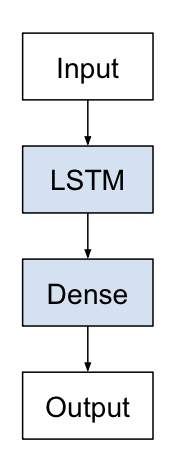
\includegraphics[width=0.2\textwidth]{images/lstm1.png}
                      \caption{Arsitektur LSTM untuk analisis data spektral \parencite{brownlee2017}.}
                      \label{fig:lstm_architecture}
                  \end{figure}

            \item \textbf{Persiapan Data Numerik} \\
                  Data numerik, seperti intensitas dan panjang gelombang, dinormalisasi untuk mempercepat pelatihan dan meningkatkan konvergensi model LSTM. Metode yang digunakan adalah Min-Max Scaling, sesuai dengan Persamaan~\eqref{eq:normalization}, dan Z-score Normalization untuk distribusi data yang lebih simetris \parencite{brownlee2017}.

            \item \textbf{Persiapan Data Kategorikal} \\
                  Data kategorikal, seperti jenis transisi atau spesies atom, diubah menjadi format numerik menggunakan One-Hot Encoding atau Label Encoding. One-Hot Encoding menghasilkan vektor biner untuk setiap kategori, sedangkan Label Encoding menetapkan nilai integer unik \parencite{brownlee2017}.

            \item \textbf{One-Hot Encoding} \\
                  One-Hot Encoding diimplementasikan menggunakan pustaka scikit-learn, seperti ditunjukkan pada Listing~\ref{lst:one_hot_encoding}:
                  \begin{lstlisting}[language=Python, caption=Contoh One-Hot Encoding dengan scikit-learn, label=lst:one_hot_encoding]
from sklearn.preprocessing import OneHotEncoder
encoder = OneHotEncoder()
encoded_data = encoder.fit_transform(data).toarray()
                  \end{lstlisting}
        \end{itemize}
\end{itemize}

\begin{theorem}
Ini adalah sebuah teorema.
\end{theorem}

\begin{definition}
Ini adalah definisi.
\end{definition}

\begin{remark}
Ini adalah catatan tanpa nomor.
\end{remark} 

\begin{proof}
Ini adalah bukti.
\end{proof}
 \begin{example}
        f
 \end{example}


 \begin{table}[H]
    \centering
    \caption{Perbandingahn  LIBS}
    \label{tab:performa_ml}
    \centering
    \begin{tabular}{lcccc}
      \toprule
      Model & Akurasi (\%) & Presisi (\%) & Recall (\%) & RMSE \\
      \midrule
      Random Forest & 95.2 & 94.8 & 95.1 & 0.12 \\
      SVM & 89.7 & 88.5 & 90.2 & 0.21 \\
      Transformer & 97.1 & 96.9 & 97.0 & 0.08 \\
      \midrule
      CNN & 93.4 & 92.7 & 93.5 & 0.15 \\
      \bottomrule
    \end{tabular}
    
    \smallskip
    \footnotesize
    \textit{Keterangan:} Data diperoleh dari 100 sampel logam dengan 5 kelas komposisi.
  \end{table}

% Baris ini digunakan untuk membantu dalam melakukan sitasi
% Karena diapit dengan comment, maka baris ini akan diabaikan
% oleh compiler LaTeX.
%\begin{comment}
%\bibliography{daftar-pustaka}
%\end{comment}
%-------------------------------------------------------------------------------
%                            BAB IV
%               		HASIL DAN PEMBAHASAN
%-------------------------------------------------------------------------------
% \fancyhf{} 
% \fancyfoot[R]{\thepage}
\chapter{HASIL DAN PEMBAHASAN}
%\thispagestyle{plain} % Halaman pertama bab menggunakan gaya plain

% Bab 4: Hasil dan Pembahasan
\chapter{Hasil dan Pembahasan}
\section{Hasil Simulasi Spektrum}
\subsection{Tingkat Energi}
[Isi Bab 4.1.1]

\subsection{Populasi Energi}
[Isi Bab 4.1.2]

\subsection{Profil Garis}
[Isi Bab 4.1.3]

\section{Prediksi dengan Transformer}
[Isi Bab 4.2: Performa dan efisiensi.]

\section{Efek Matriks}
[Isi Bab 4.3: Simulasi dan mitigasi.]

\section{Analisis LTE}
[Isi Bab 4.4: Sensitivitas deviasi.]

\section{Perbandingan Penelitian}
[Isi Bab 4.5: Keunggulan kuantum-Transformer.]

\section{Implikasi}
[Isi Bab 4.6: Teoritis dan praktis.]


\begin{table}[H]
    \centering
    \caption{Hasil Pengujian Akurasi Menggunakan SVM Terhadap Data \textit{Training} dan \textit{Testing}}
    \label{tb_detail_akurasi_face}
    \begin{tabular}{lcccc}
    \toprule
    \textbf{Jenis Data} & \textbf{Jumlah Label} & \textbf{Jumlah Data} & {\color[HTML]{000000} \textbf{Akurasi}} \\ 
    \midrule
    {\color[HTML]{000000} Training} & {\color[HTML]{000000} 41} & {\color[HTML]{000000} 1640} & {\color[HTML]{000000} 99,51\%} \\ 
    {\color[HTML]{000000} Testing} & {\color[HTML]{000000} 41} & {\color[HTML]{000000} 410} & {\color[HTML]{000000} 96,34\%} \\ 
    \bottomrule
    \end{tabular}
    \end{table}

    \begin{table}[H]
        \centering
        \caption{Perbandingan Performa Model Performa Model Performa Model Performa Model Machine Learning pada Data LIBS}
        \label{tab:performa_ml}
        \centering
        \begin{tabular}{lcccc}
          \toprule
          Model & Akurasi (\%) & Presisi (\%) & Recall (\%) & RMSE \\
          \midrule
          Random Forest & 95.2 & 94.8 & 95.1 & 0.12 \\
          SVM & 89.7 & 88.5 & 90.2 & 0.21 \\
          Transformer & 97.1 & 96.9 & 97.0 & 0.08 \\
          CNN & 93.4 & 92.7 & 93.5 & 0.15 \\
          \bottomrule
        \end{tabular}
        
        \smallskip
        \footnotesize
        \textit{Keterangan:} Data diperoleh dari 100 sampel logam dengan 5 kelas komposisi.
      \end{table}
    

% Baris ini digunakan untuk membantu dalam melakukan sitasi
% Karena diapit dengan comment, maka baris ini akan diabaikan
% oleh compiler LaTeX.
\begin{comment}
\bibliography{daftar-pustaka}
\end{comment}
%-------------------------------------------------------------------------------
%                            BAB V
%               		KESIMPULAN DAN SARAN
%-------------------------------------------------------------------------------
% \fancyhf{} 
% \fancyfoot[R]{\thepage}
\chapter{KESIMPULAN DAN SARAN}
%\thispagestyle{plain} % Halaman pertama bab menggunakan gaya plain

\section{Kesimpulan}

\section{Saran}


%-----------------------------------------------------------------------------%

% Baris ini digunakan untuk membantu dalam melakukan sitasi
% Karena diapit dengan comment, maka baris ini akan diabaikan
% oleh compiler LaTeX.
\begin{comment}
\bibliography{daftar-pustaka}
\end{comment}

\fancypagestyle{daftarpustaka}{
  \fancyhf{}
  \fancyfoot[R]{\thepage}
  \renewcommand{\headrulewidth}{0pt}
  \renewcommand{\footrulewidth}{0pt}
}

\addcontentsline{toc}{chapter}{DAFTAR PUSTAKA}
\begin{onehalfspace}
  \begin{spacing}{1}
    \pagestyle{daftarpustaka}
  \end{spacing}
  \bibliography{daftar-pustaka}
\end{onehalfspace}

% File: include/lampiran.tex
% Lampiran untuk Tugas Akhir Jurusan Informatika Unsyiah
% Sesuai Panduan Tugas Akhir dan Tesis 2024 FMIPA Universitas Syiah Kuala
% Struktur: Hanya Lampiran 1, 2, dst., tanpa subbab atau section

% \begin{onehalfspace} % Spasi 1,5 sesuai dokumen utama

\lampiran{Algoritma Inisialisasi Data Spektral Atom}
\label{app:algo1}
\begin{algoritma}[H]
\small
\caption{Inisialisasi Data Spektral Atom}
\begin{algorithmic}[1]
  \REQUIRE Transition dataset $\mathcal{D} = \{ (\lambda_{ij}, E_i, E_k, g_i, g_k, A_{ki}) \mid \lambda_{ij} \in [200, 900], E_i, E_k, g_i, g_k, A_{ki} > 0 \}$ ; Number of element-ion pairs $k = 4$; Maximum spectral samples $N \in \mathbb{N}$; Temperature step $\Delta T > 0$; Electron density step $\Delta n_e > 0$
  \ENSURE Candidate atom set $\mathcal{C}$, atom subset dictionary $\mathcal{A}$, spectra set $\mathcal{S}$
  \STATE Validate inputs: Ensure $N > 0$, $\Delta T > 0$, $\Delta n_e > 0$
  \STATE Initialize: $\Delta T \gets 1000$, $\Delta n_e \gets 10^{0.5} \times 10^{12}$
  \STATE Define: $\mathcal{C} \gets \{\text{H}, \text{He}, \text{O}, \text{N}, \text{Si}, \text{Al}, \text{Fe}, \text{Ca}, \text{Mg}, \text{Na}, \text{Ti}, \text{Mn}, \text{S}, \text{Cl}, \text{Cr}, \text{Ni}, \text{Cu}\}$
  \STATE Initialize: $\mathcal{S} \gets \emptyset$, $\mathcal{A} \gets \emptyset$
  \FORALL{$T \in [5000, 15000]$ \textbf{step} $\Delta T$}
    \FORALL{$n_e \in [10^{12}, 10^{16}]$ \textbf{step} $\Delta n_e$}
      \STATE Randomly select $\mathcal{A}_{T,n_e} \subseteq \mathcal{C}$ with $|\mathcal{A}_{T,n_e}| = k$ without replacement
      \IF{no transitions exist in $\mathcal{D}$ for any species in $\mathcal{A}_{T,n_e}$}
        \STATE Log warning: ``No transitions for $\mathcal{A}_{T,n_e}$ at $T$, $n_e$'' \COMMENT{Skip}
        \STATE continue
      \ENDIF
      \STATE Store $(T, n_e, \mathcal{A}_{T,n_e})$ in $\mathcal{A}$
    \ENDFOR
  \ENDFOR
  \RETURN $\mathcal{C}$, $\mathcal{A}$, $\mathcal{S}$
\end{algorithmic}
\end{algoritma}
% Algoritma ini mengumpulkan dan memvalidasi data transisi atom dari basis data NIST, menginisialisasi set kandidat atom (\(\mathcal{C}\)), kamus subset atom (\(\mathcal{A}\)), dan set spektrum (\(\mathcal{S}\)). Subset atom dipilih secara acak untuk setiap kombinasi \(T\) dan \(n_e\), memastikan representasi yang beragam.

\lampiran{Algoritma Kalkulasi Rasio Populasi Ionisasi}
\label{app:algo2}
\begin{algoritma}[h]
\small
\caption{Kalkulasi Rasio Populasi Ionisasi}
\begin{algorithmic}[1]
  \REQUIRE Transition dataset $\mathcal{D} = \{ (\lambda_{ij}, E_i, E_k, g_i, g_k, A_{ki}) \mid \lambda_{ij} \in [200, 900], E_i, E_k, g_i, g_k, A_{ki} > 0 \}$; \\ Candidate atom set $\mathcal{C}$; \\ Atom subset dictionary $\mathcal{A} = \{ (T, n_e, \mathcal{A}_{T,n_e}) \}$; \\ Physical constants $m_e = 9.109 \times 10^{-31}$, $k_B = 8.617 \times 10^{-5}$, $h = 4.1357 \times 10^{-15}$
  \ENSURE Population ratio dictionary $\mathcal{R} = \{ (T, n_e, \mathbf{R}_{T,n_e}) \mid \mathbf{R}_{T,n_e} \in [0, 1]^2 \}$
  \STATE Initialize $\mathcal{R} \gets \emptyset$ \COMMENT{Ratio dictionary}
  \FORALL{$(T, n_e, \mathcal{A}_{T,n_e}) \in \mathcal{A}$}
    \STATE $\mathbf{R}_{T,n_e} \gets \emptyset$ \COMMENT{Temporary ratio}
    \FORALL{$S \in \mathcal{A}_{T,n_e}$}
      \STATE Define $(S_{\text{neutral}}, S_{\text{ion}}) \gets (S_{\text{neutral}}, S_{\text{ion}})$ \COMMENT{Species pair}
      \STATE Extract $\mathcal{T}_S \subseteq \mathcal{D}$ for $S_{\text{neutral}}$ or $S_{\text{ion}}$ \COMMENT{Transitions}
      \IF{$\mathcal{T}_S = \emptyset$}
        \STATE Log warning: ``No transitions for $S$'' \COMMENT{Skip}
        \STATE continue
      \ENDIF
      \STATE $Z_{\text{neutral}} \gets \sum_i g_i \exp\left(-\frac{E_i}{k_B T}\right)$ \COMMENT{Neutral partition}
      \IF{$Z_{\text{neutral}} \leq 0$}
        \STATE Log warning: ``Invalid partition function for $S_{\text{neutral}}$'' \COMMENT{Skip}
        \STATE continue
      \ENDIF
      \STATE $Z_{\text{ion}} \gets \sum_i g_i \exp\left(-\frac{E_i}{k_B T}\right)$ \COMMENT{Ion partition}
      \IF{$Z_{\text{ion}} \leq 0$}
        \STATE Log warning: ``Invalid partition function for $S_{\text{ion}}$'' \COMMENT{Skip}
        \STATE continue
      \ENDIF
      \STATE $\frac{N_{\text{ion}}}{N_{\text{neutral}}} \gets \frac{2 Z_{\text{ion}}}{n_e Z_{\text{neutral}}} \left( \frac{2\pi m_e k_B T}{h^2} \right)^{3/2} \exp\left(-\frac{E_{\text{ion}}}{k_B T}\right)$ \COMMENT{Ionization ratio}
      \STATE $f_{\text{neutral}} \gets \frac{1}{1 + \frac{N_{\text{ion}}}{N_{\text{neutral}}}}$ \COMMENT{Neutral fraction}
      \STATE $f_{\text{ion}} \gets \frac{\frac{N_{\text{ion}}}{N_{\text{neutral}}}}{1 + \frac{N_{\text{ion}}}{N_{\text{neutral}}}}$ \COMMENT{Ion fraction}
      \STATE Store $(f_{\text{neutral}}, f_{\text{ion}})$ in $\mathbf{R}_{T,n_e}[S_{\text{neutral}}, S_{\text{ion}}]$ \COMMENT{Store ratio}
    \ENDFOR
    \STATE Store $(T, n_e, \mathbf{R}_{T,n_e})$ in $\mathcal{R}$ \COMMENT{Add to dictionary}
  \ENDFOR
  \RETURN $\mathcal{R}$ \COMMENT{Result}
\end{algorithmic}
\end{algoritma}
% Algoritma ini menghitung rasio populasi ionisasi untuk setiap pasangan elemen-ion, menghasilkan kamus rasio populasi (\(\mathcal{R}\)). Rasio ini penting untuk menentukan fraksi atom netral dan terionisasi dalam plasma.

\lampiran{Algoritma Kalkulasi Intensitas Garis Spektral}
\label{app:algo3}
\begin{algoritma}[H]
\small
\caption{Kalkulasi Intensitas Garis Spektral}
\begin{algorithmic}[1]
  \REQUIRE Transition dataset $\mathcal{D} = \{ (\lambda_{ij}, E_i, E_k, g_i, g_k, A_{ki}, m_a, w) \mid \lambda_{ij} \in [200, 900], E_i, E_k, g_i, g_k, A_{ki}, m_a, w > 0 \}$; \\ Atom subset dictionary $\mathcal{A} = \{ (T, n_e, \mathcal{A}_{T,n_e}) \}$; \\ Population ratio dictionary $\mathcal{R} = \{ (T, n_e, \mathbf{R}_{T,n_e}) \mid \mathbf{R}_{T,n_e} \in [0, 1]^2 \}$; \\ Physical constants $c = 2.998 \times 10^8$, $k_B = 8.617 \times 10^{-5}$
  \ENSURE Temporary intensity dictionary $\mathcal{I} = \{ (T, n_e, \mathbf{I}_{\text{temp}}) \mid \mathbf{I}_{\text{temp}} = \{ (\lambda_{ij}, I_{\text{rel}}) \} \}$
  \STATE Initialize $\mathcal{I} \gets \emptyset$ \COMMENT{Temporary intensity dictionary}
  \FORALL{$(T, n_e, \mathcal{A}_{T,n_e}) \in \mathcal{A}$}
    \STATE Extract $\mathbf{R}_{T,n_e}$ from $\mathcal{R}$ \COMMENT{Population ratio}
    \STATE $\mathbf{I}_{\text{temp}} \gets \emptyset$ \COMMENT{Temporary intensity list}
    \FORALL{$S \in \mathcal{A}_{T,n_e}$}
      \STATE Extract $\mathcal{T}_S \subseteq \mathcal{D}$ for $S_{\text{neutral}}$ or $S_{\text{ion}}$ \COMMENT{Transitions}
      \IF{$\mathcal{T}_S = \emptyset$}
        \STATE Log warning: ``No transitions for $S$'' \COMMENT{Skip}
        \STATE continue
      \ENDIF
      \FORALL{$(\lambda_{ij}, E_i, E_k, g_i, g_k, A_{ki}, m_a, w) \in \mathcal{T}_S$}
        \STATE $\Delta E \gets E_k - E_i$ \COMMENT{Energy}
        \STATE $n_{e,\text{min}} \gets 1.6 \times 10^{12} T^{1/2} (\Delta E)^{3/2}$ \COMMENT{Minimum density}
        \IF{$n_e \geq n_{e,\text{min}}$}
          \IF{$S$ is $S_{\text{neutral}}$}
            \STATE $Z \gets Z_{\text{neutral}}$ (Algoritma 2) \COMMENT{Neutral partition}
            \STATE $f \gets f_{\text{neutral}}$ from $\mathbf{R}_{T,n_e}$ \COMMENT{Neutral fraction}
          \ELSE
            \STATE $Z \gets Z_{\text{ion}}$ (Algoritma 2) \COMMENT{Ion partition}
            \STATE $f \gets f_{\text{ion}}$ from $\mathbf{R}_{T,n_e}$ \COMMENT{Ion fraction}
          \ENDIF
          \STATE $I_{\text{rel}} \gets \frac{g_k A_{ki} \exp\left(-\frac{E_k}{k_B T}\right)}{Z} \cdot f$ \COMMENT{Relative intensity}
          \STATE Append $(\lambda_{ij}, I_{\text{rel}})$ to $\mathbf{I}_{\text{temp}}$ \COMMENT{Accumulate}
        \ELSE
          \STATE Log warning: ``LTE condition not satisfied'' \COMMENT{Skip}
        \ENDIF
      \ENDFOR
    \ENDFOR
    \STATE Store $(T, n_e, \mathbf{I}_{\text{temp}})$ in $\mathcal{I}$ \COMMENT{Add to dictionary}
  \ENDFOR
  \RETURN $\mathcal{I}$ \COMMENT{Result}
\end{algorithmic}
\end{algoritma}
% \par Algoritma ini menghitung intensitas relatif garis spektral (\(I_{\text{rel}}\)) untuk setiap transisi atom, menghasilkan kamus intensitas sementara (\(\mathcal{I}\)). Intensitas ini mencerminkan probabilitas emisi foton.

\lampiran{Algoritma Kalkulasi Spektrum Emisi dengan Profil Voigt}
\label{app:algo4}
\begin{algoritma}[H]
\small
\caption{Kalkulasi Spektrum Emisi Atom dengan Profil Garis \textit{Voigt}}
\begin{algorithmic}[1]
  \REQUIRE Temporary intensity dictionary $\mathcal{I} = \{ (T, n_e, \mathbf{I}_{\text{temp}}) \mid \mathbf{I}_{\text{temp}} = \{ (\lambda_{ij}, I_{\text{rel}}) \} \}$; \\ Transition dataset $\mathcal{D} = \{ (\lambda_{ij}, E_i, E_k, g_i, g_k, A_{ki}, m_a, w) \mid \lambda_{ij} \in [200, 900], E_i, E_k, g_i, g_k, A_{ki}, m_a, w > 0 \}$; \\ Atom subset dictionary $\mathcal{A} = \{ (T, n_e, \mathcal{A}_{T,n_e}) \}$; \\ Population ratio dictionary $\mathcal{R} = \{ (T, n_e, \mathbf{R}_{T,n_e}) \mid \mathbf{R}_{T,n_e} \in [0, 1]^2 \}$; \\ Physical constants $c = 2.998 \times 10^8$, $k_B = 8.617 \times 10^{-5}$; \\ Maximum spectral samples $N \in \mathbb{N}$; \\ Spectra set $\mathcal{S}$
  \ENSURE $\mathcal{S}$ with $(T, n_e, \mathbf{I}_{T,n_e}, \mathbf{R}_{T,n_e})$
  \STATE Initialize $c \gets 0$ \COMMENT{Counter}
  \FORALL{$(T, n_e, \mathbf{I}_{\text{temp}}) \in \mathcal{I}$}
    \STATE Extract $\mathbf{R}_{T,n_e}$ from $\mathcal{R}$ \COMMENT{Population ratio}
    \STATE $\mathbf{I}_{T,n_e} \gets \emptyset$ \COMMENT{Final intensity list}
    \FORALL{$(\lambda_{ij}, I_{\text{rel}}) \in \mathbf{I}_{\text{temp}}$}
      \STATE Extract $m_a, w$ from $\mathcal{D}$ for the transition at $\lambda_{ij}$ \COMMENT{Atom mass and Lorentzian width}
      \STATE $\alpha_G \gets \frac{\lambda_{ij}}{c} \sqrt{\frac{2 k_B T \ln 2}{m_a}}$ \COMMENT{Gaussian HWHM (Doppler)}
      \STATE $\alpha_L \gets w \cdot \frac{n_e}{10^{16} \sqrt{T}}$ \COMMENT{Lorentzian HWHM}
      \STATE $I(\lambda) \gets I_{\text{rel}} \cdot V(\lambda - \lambda_{ij}, \alpha_G, \alpha_L)$ \COMMENT{Voigt profile}
      \STATE Append $(\lambda_{ij}, I(\lambda))$ to $\mathbf{I}_{T,n_e}$ \COMMENT{Accumulate}
    \ENDFOR
    \IF{$\max(\{I \mid (\lambda_{ij}, I) \in \mathbf{I}_{T,n_e}\}) > 0$}
      \STATE Normalize $\mathbf{I}_{T,n_e}$: divide each $I$ by $\max(\{I \mid (\lambda_{ij}, I) \in \mathbf{I}_{T,n_e}\})$ \COMMENT{Normalization}
    \ENDIF
    \STATE Store $(T, n_e, \mathbf{I}_{T,n_e}, \mathbf{R}_{T,n_e})$ in $\mathcal{S}$ \COMMENT{Add spectrum}
    \STATE $c \gets c + 1$ \COMMENT{Increment}
    \IF{$c \mod 1000 = 0$} %\COMMENT{Check storage modulo}
      \STATE Save $\mathcal{S}$ \COMMENT{Save}
      \STATE Clear $\mathcal{S}$ \COMMENT{Clear}
    \ENDIF
    \IF{$c \geq N$}
      \STATE break \COMMENT{Terminate}
    \ENDIF
  \ENDFOR
  \RETURN $\mathcal{S}$ \COMMENT{Result}
\end{algorithmic}
\end{algoritma}
% Algoritma ini menghitung parameter pelebaran Gaussian (\(\alpha_G\)) dan Lorentzian (\(\alpha_L\)), lalu mengaplikasikan profil Voigt untuk menghasilkan spektrum emisi akhir, menyimpannya dalam set spektrum (\(\mathcal{S}\)) dengan normalisasi intensitas.

% % \end{onehalfspace}
\addcontentsline{toc}{chapter}{LAMPIRAN}

\end{onehalfspace}
\end{document}